\chapter{Building Applications}
\label{ch:apps}

Tendermint is designed to be a general purpose algorithm for replicating a deterministic state machine.
It uses the Tendermint Socket Protocol (TMSP) to standardize communication between the consensus engine and the state machine,
enabling application developers to build their state machines in any programming language, 
and have it automatically replicated via Tendermint's BFT algorithm.

\section{Background}

Applications on the internet can in general be characterized as containing two fundamental components:

\begin{itemize}
\item{Engine: handles core security, networking, replication functionality. Typically a webserver, like Apache or NginX, when powering a web app, or a consensus algorithm when powering a distributed application}
\item{State-machine: the actual application code that processes transactions received from the engine  and updates internal state}
\end{itemize}

This separation of concerns enables application developers to write state-machines in any programming language representing arbitrary applications,
on top of an engine which may be specialized for its performance, security, useability, support, etc.

Unlike web-servers and their applications, which often take the form of processes communicating over a socket via the Common Gateway Interface (CGI) protocol,
consensus algorithms have traditionally had much less useable or less general purpose interfaces to build applications on top of.
Some, like zookeeper, etcd, consul, and other distributed key-value stores, 
provide HTTP interfaces to a particular instance of a simple key-value application, 
with some more interesting features like atomic compare-and-swap operations and push notificaitons.
But they do not give the application developer control of the state-machine code itself.

Demand for such a high-level of control over the state-machine running above a consensus engine has been driven primarily by the success of Bitcoin and the consequent interest in blockchain technology.
By building more advanced applications directly into the consensus, 
users, developers, regulators, etc. can achieve greater security gaurantees on arbitrary state-machines, 
far beyond key-value stores, like currencies, exchanges, supply-chain management, governance, and so on.

What has so captured the attention of so many is the potential of a system which permits collective enforcement of the execution of code.
It is practically a re-invention of many dimensions of the legal system, using distribtued consensus algorithms and deterministically executable contracts,
rather than policemen, lawyers, judges, juries, and the like.
The ramifications for the development of human society are expolisive, much as the introduction of the democratic rule of law was in the first place.

Tendermint aims to provide the fundamental interface and consensus engine upon which such applications might be built.

\section{Tendermint Socket Protocol}

The Tendermint Socket Protocol (TMSP) defines the core interface by which the consensus engine communicates with the application state machine.
The interface definition consists of a number of message types, specified using Google's Protobuf \cite{protobuf}, 
that are length-prefixed and transmitted over a socket \ref{fig:tmsp}.

\begin{figure}[]
	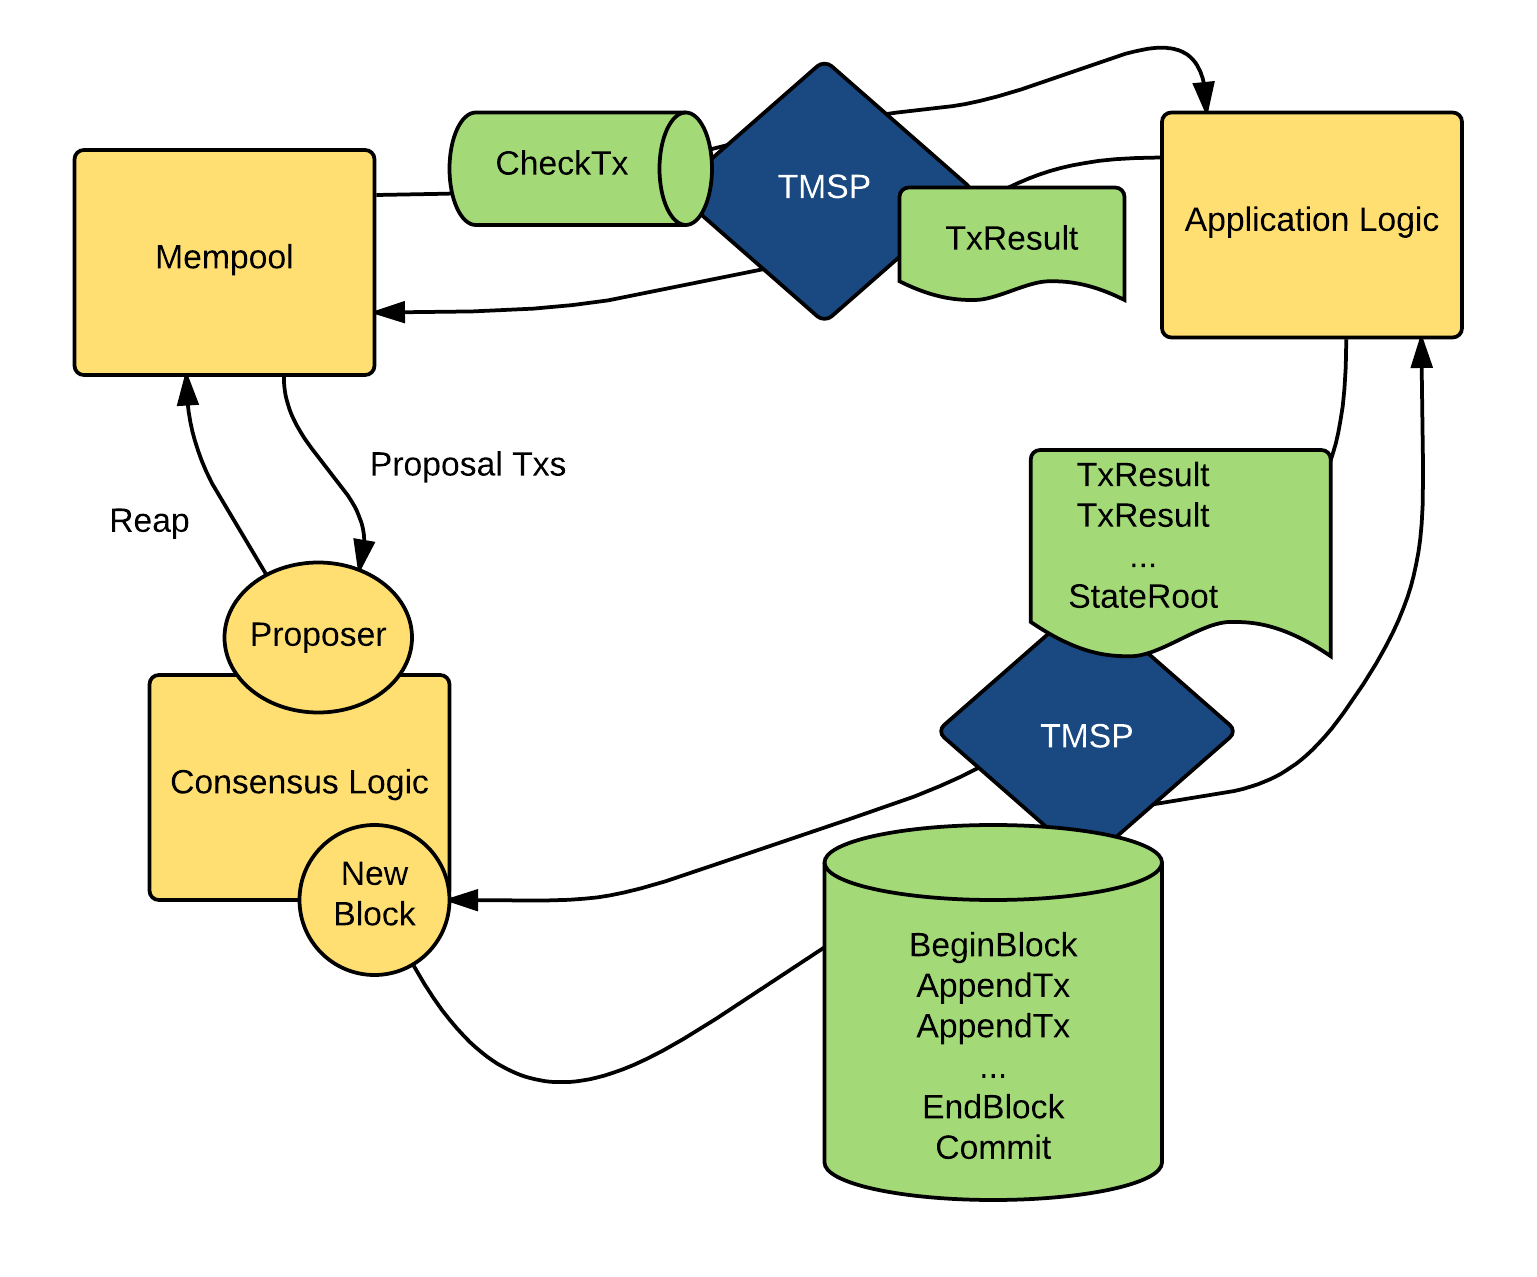
\includegraphics[width=\linewidth,height=\textheight,keepaspectratio]{figures/tmsp.png}
    	\centering
	\label{fig:tmsp}
	\caption[TMSP Architecture]{
The consensus logic communicates with the application logic via TMSP, a socket protocol. 
Two sockets are maintained, one for the mempool to check the validity of new transactions,
and one for the consensus to execute newly committed blocks.
}
\end{figure}

TMSP is implemented as a fully asynchronous server, 
where message types come in pairs of request and response,
and where a special message type, Flush, pushes any buffered messages over the connection and awaits all responses.

At the core of the TMSP are two messages: \emph{AppendTx} and \emph{Commit}.
Once a block is committed by the consensus, 
the engine calls AppendTx on each transaction in the block, 
passing it to the application state-machine to be processed.
If the transaction is valid, it will result in a state-transition in the application.

Once all AppendTx calls have returned, the consensus engine calls Commit,
causing the application to commit to the latest state, and persist it to disk.

\section{Separating Agreement and Execution}

Using the TMSP affords us an explicit separation between consensus, or agreement on the order of transactions, 
and their actual execution in the state-machine.
In particular, we achieve consensus on the order first, and then execute the ordered transactions.
This separation actually improves the system's fault tolerance \cite{yin2003separating}:
while $3f+1$ replicas are still needed for agreement to tolerate $f$ Byzantine failures, 
only $2f+1$ replicas are needed for execution.
That is, while we still need a two-thirds majority for ordering, we only need a one-half majority for execution.

On the other hand, the fact that transactions are executed after they are ordered results in possibly invalid transactions,
which can waste system resources. 
This is solved using an additional TMSP message, \emph{CheckTx}, which is called by the mempool,
allowing it to check whether the transaction would be valid against the latest state.
Note, however, that the fact that commits come in blocks at a time introduces complexity in the handling of CheckTx messages.
In particular, applications are expected to maintain a second state-machine that executes only those rules of the main state-machine pertaining to a transaction's validity. 
This second state-machine is updated by CheckTx messages and is reset to the latest committed state after every commit.
In essence, the second state machine describes the transaction pool's filter rules.

To some extent, CheckTx can be used as an optimistic execution, 
returning a result to the transaction sender with the caveat that 
the result may be wrong if a block is committed with a conflicting transaction
before the transaction of interest is committed.
This sort of optimistic execution is the focus of an approach to scalable BFT systems 
that can work quite well for particular applications where conflicts between transactions are rare. 
At the same time, it adds additional complexity to the client, by virtue of needing to handle possibly invalid results.
The approach is discussed further in Chapter \ref{ch:related}.

\section{Microservice Architecture}

Adopting separation of concerns as a strategy in application design is generally considered wise practice \ref{hursch1995separation}.
In particular, many large scale application deployments today adopt a microservice architecture,
wherein each functional component is implemented as a standalone network service, 
and typically encapsulated in a linux container (eg. using Docker) for efficient deployment, scalability, and upgradeability.

Applications running above Tendermint consensus will often be decomposable into microservices.
For instance, many applications will utilize a key-value store for storing state.
Running the key-value store as an independent service is quite common, 
in order to take advantage of the data store's specialized features, such as high-performance data types or merklization.

Another important microservice for applications is a governance module, 
which manages a certain subset of TMSP messages, enabling the application to control validator set changes.
Such a module can become a powerful paradigm for governance in BFT systems.

Some applications may utilize a native currency or account structure for users.
It may thus be useful to provide a module which supports basic elements of, for instance,
handling digital signatures and managing account dynamics.

The list of possible microservices to compose a complex TMSP applications goes on. 
In fact, one might even build an application which can launch sub-applications using data sent in transactions.
For instance, including the hash of a docker image in a transaction,
such that the image could be pulled from some file-storage backend and run as a sub-application where
future transactions in the consensus could cause it to execute. 
This is the approach of ethereum, 
which allows developers to deploy bits of code to the network that can be triggered to run within the ethereum virtual machine by future transactions \cite{ethereum},
and of IBM's recent OpenBlockChain (OBC) project, which allows developers to send full docker contexts in transactions, 
defining containers that run arbitrary code in response to transactions addressed to them \cite{obc}.

\section{Determinism}

The most critical caveat about building applications using TMSP is that they must be deterministic.
That is, for the replicated state-machine to not compromise safety, 
every node must obtain the same result when executing the same transaction against the same state.

This is not a unique requirement for Tendermint. Bitcoin, Raft, Ethereum, any other distributed consensus algorithm,
and applications like lock-step multiplayer gaming must all be strictly deterministic, lest a consensus failure arise,
or a desynchronisation, as its called in the gaming world.

There are many sources of non-determinism in programming languages, most obviously via random numbers and time,
but also, for instance, via the use of floats, and by iteration over hash tables 
(some languages, such as Go, enforce randomized iteration over hash tables to force programmers to be explicit about when they need ordered data structures).
The strict restriction on determinism, and its notable lacking from every major programming language,
prompted ethereum to develop its own, Turing-complete, fully deterministic virtual machine,
which forms the platform for application developers to build applications above the ethereum blockchain.
While deterministic, it has many quirks, such as 32-byte stack words, storage keys, and storage values,
and no support for byte-shifting operations - everything is big number arithmetic.

Deterministic programming is well studied in the world of real-time, lockstep, multi-party gaming.
Such games constitute another example of replicated state machines, and are quite similar in many ways to consensus algorithms.
Application developers building with TMSP are encouraged to study their methods, and to take care when implementing an application.
On the one hand, the use of functional programming languages and proof methods can enable the construction of correct programs.
On the other, compilers are being built to translate possibly non-deterministic programs to canonically deterministic ones \cite{deterministicjs}.

\section{Termination}

If determinism is critical for preserving safety, termination of transaction execution is critical for preserving liveness.
It is, however, not in general possible to determine whether a given program halts for even a single input, let alone all of them,
a problem known as the Halting Problem \cite{halting}.

Ethereum's virtual machine solves the problem by \emph{metering}, that is, charging for each operation in the execution.
This way, a transaction is gauranteed to terminate when the sender runs out of funds.
Such metering may be possible in a more general case, 
via compilers that compile programs to metered versions of themselves \cite{} (CITE GREG).

It is difficult to solve this problem without significant overhead.
In essence, a validator cannot tell if an execution is in an infinite loop or is just slow, but nearly complete.
It may be possible to use the Tendermint consensus protocol to decide on transaction timeouts, 
such that more than two-thirds of validators must agree that a transaction timed out and is thus considered invalid (ie. having no effect on the state)
However, we do not pursue the idea further here, leaving it to future work. 
In the meantime, it is expected that applications will undergo thorogh testing before being deployed in any consensus system,
and that monitoring and governance mechanisms will be used to resurrect the system in the event of consensus failure.

\section{Examples}

\subsection{Merkleeyes}

A simple example of a tmsp application is a merklized key-value store. 
Tendermint provides merkleeyes, a tmsp application which wraps a self-balancing, merkle binary search tree.
The first byte of a transaction determines if the transation is a get, set, or remove operation. 
For get and remove operations, the remaining bytes are the key. 
For the set operation, the remaining bytes are a serialized list containing the key and value.
Merkleeyes may utilize a simple implementation of CheckTx that only decodes the transaction,
to ensure it is properly formatted.
One could also make a more advanced CheckTx, where get and remove operations on unknown keys are invalid.
Once Commit is called, the latest updates are added into the merkle tree, all hashes are computed, 
and the latest state of the tree is committed to disk.

Note that Merkleeyes was designed to be a module used by other tmsp applications for a merklized key-value store,
rather than a stand alone tmsp application, though the simplicity of the tmsp interface makes it ammenable to both.

\subsection{Basecoin}

A more complete example is a simple currency, 
using an account structure pioneered by Ethereum, 
where each user has a public key and an account with the balance for that public key.
The account also contains a sequence number, which is equal to the number of transactions sent by the account.
Transactions can send funds from the account if they include the correct sequence number
and are signed by the correct private key.
Without the sequence number, the system would be susceptible to replay attacks,
where a signed transaction debitting an account could be replayed, 
causing the debit to occur multiple times.

An application supporting a currency has naturally more logic than a simple key-value store.
In particular, certain transactions are distinctly invalid, 
such as those with an invalid signature, incorrect sequence number,
or sending an amount greater than the sender's account balance.
These conditions can be checked in CheckTx.

Furthermore, a suplementary application state must be maintained for CheckTx 
in order to update sequence numbers and account balances 
when there are multiple transactions involving the same accounts in the mempool at once.
When commit is called, the suplementary application state is reset to the latest committed state.
Any transactions still in the mempool can be replayed via CheckTx against the latest state.

\subsection{Ethereum}

Ethereum uses the mechanisms already described to filter transactions out of the mempool,
but it also runs some transactions in a virtual machine, 
which updates state and returns results.
The virtual machine execution is not done in CheckTx, 
as it is much more expensive and depends heavily on the ultimate order of transactions as they are included in blocks.

\section{Conclusion}

TMSP provides a simple yet flexible means to build arbitrary applications,
in any programming language,
that inherit BFT state-machine replication from the Tendermint consensus algorithm.
It plays much the same role for a consensus engine and an application that, for instance, CGI plays for Apache and Wordpress.
However, application developers must take special care to ensure their applications are deterministic, and that transaction executions terminate.

